We are interested in the dynamics that emerge when fixing the parameters $\beta = 1, f = 150, L = 4.2 \cdot 10^{-3}, R = 2, V_m = 5,$ and $\mu = 0.5$.
The parameters $E_0$ and $\chi_0$ are varied.
$E_0$ is in the range $[14, 28]$, while $\chi_0$ is in the range $[0.1, 0.65]$.
When scanning this parameter plane for the period of emerging cycles, \Cref{fig:yunus.2pi.2d.full} emerges.

\begin{figure}
    \centering
    \includegraphics[width=0.6\textwidth]{99_Yunus/2D_Period/result.png}
    \caption{2D Scan of Original Model}
    \label{fig:yunus.2pi.2d.full}
\end{figure}

The thing, we are interested in, is what happens along the red line.
The period stays the same, but the area, where this period is, gets thinner at this point.
\Cref{fig:yunus.2pi.CobwebA2,fig:yunus.2pi.CobwebB2} show what happens right at the beginning of the thin area.
When you follow the blue line in \Cref{fig:yunus.2pi.CobwebB2}, you see that there are two cycles of period 12 coexisting.
In \Cref{fig:yunus.2pi.CobwebA2} there was only one cycle of period 12 and it still exists in \Cref{fig:yunus.2pi.CobwebB2}.
Its symbolic sequence is $\A^3\B^3\C^3\D^3$.
The symbolic sequence of the new cycle in \Cref{fig:yunus.2pi.CobwebB2} is $\A^2\B^4\C^2\D^4$.

\begin{figure}
    \centering
    \begin{subfigure}{0.4\textwidth}
        \centering
        \includegraphics[width=\textwidth]{99_Yunus/Period12/Cobweb_A2/result.png}
        \caption{Cobweb before the thin area begins}
        \label{fig:yunus.2pi.CobwebA2}
    \end{subfigure}
    \begin{subfigure}{0.4\textwidth}
        \centering
        \includegraphics[width=\textwidth]{99_Yunus/Period12/Cobweb_B2/result.png}
        \caption{Cobweb after the thin area begins}
        \label{fig:yunus.2pi.CobwebB2}
    \end{subfigure}
\end{figure}
